% !TEX program = xelatex
\documentclass[12pt,a4paper]{article}
\usepackage[utf8]{inputenc}
\usepackage{graphicx}
\usepackage{hyperref}
\usepackage{float}
\usepackage{geometry}
\usepackage{xcolor}
\usepackage{setspace}
\usepackage{fancybox}
\usepackage{listings}
\usepackage{amsmath}
\usepackage{booktabs}
\usepackage{minted}

% Define professional colors
\definecolor{highlight}{RGB}{42, 53, 227}  % Deep blue for highlights
\definecolor{accent}{RGB}{42, 53, 227}    % Deep blue for accents


% Page geometry
\geometry{
    a4paper,
    margin=1.5cm,
    includehead,
    includefoot
}

\begin{document}

% Title Page
\begin{titlepage}
\thispagestyle{empty}

% Calculate margins for centering the box
\newlength{\boxwidth}
\setlength{\boxwidth}{\textwidth}
\addtolength{\boxwidth}{-4mm}\setlength{\fboxrule}{2pt}

\newlength{\boxheight}
\setlength{\boxheight}{\textheight}
\addtolength{\boxheight}{1.9cm}

\centering
\vspace*{-2.5cm}
\fbox{%
\begin{minipage}[c][\boxheight][s]{\boxwidth}
\begin{center}


\vspace{12cm}
{\huge\textbf{\color{highlight}Digital Pulse-Coded\\Laser Authentication System}\par}
\vspace{1cm}

\end{center}
\end{minipage}
}
\end{titlepage}

% Table of Contents
\tableofcontents
\newpage

\section*{Abstract}
This project implements a contactless digital authentication system utilizing modulated laser pulses for access control applications. The system employs an 8-bit binary sequence transmitted via a 650nm laser diode and detected by a dedicated laser sensor, demonstrating the practical application of optical physics principles in modern security solutions. The implementation achieves reliable authentication while maintaining cost-effectiveness through the use of readily available components.

\section{Introduction}
\subsection{Background}
Traditional authentication systems often rely on physical contact or radio frequency (RF) communication, each presenting their own limitations. Physical contact systems are subject to wear and contamination, while RF systems can be vulnerable to interference and interception. Optical authentication offers an alternative approach that combines the benefits of contactless operation with directed, line-of-sight security.

\subsection{Project Objectives}
\begin{itemize}
    \item Design and implement a contactless authentication system using laser-based communication
    \item Achieve reliable signal transmission and detection under normal indoor lighting conditions
    \item Optimize the timing parameters for practical usage while maintaining system integrity
    \item Demonstrate the feasibility of low-cost optical authentication using common components
\end{itemize}

\section{System Architecture}
\subsection{Hardware Components}
\subsubsection{Transmission Module}
\begin{itemize}
    \item 650nm laser diode module
    \item microcontroller
    \item Power supply: USB connection via Arduino
\end{itemize}

\subsubsection{Reception Module}
\begin{itemize}
    \item Laser sensor module with built-in signal conditioning
    \item Arduino analog input for signal processing
    \item Status LEDs (Red and Green) with appropriate current-limiting resistors
\end{itemize}

\subsection{Authentication Protocol}
The system implements an 8-bit authentication sequence:
\begin{itemize}
    \item Binary pattern: [1, 0, 1, 1, 0, 0, 1, 1]
    \item Optimized timing parameters:
    \begin{itemize}
        \item Pulse width: 100ms (HIGH state duration)
        \item Bit interval: 200ms (total time per bit)
        \item Complete sequence duration: $\sim$1.6 seconds
    \end{itemize}
\end{itemize}

\section{Implementation Details}
\subsection{Signal Generation}
The transmission module generates precisely timed laser pulses using the following parameters:
\begin{minted}{arduino}
const unsigned long pulseWidth = 100;    // Active pulse duration (ms)
const unsigned long bitInterval = 200;   // Time between pulse starts (ms)
const unsigned long readInterval = 20;   // Sensor sampling interval (ms)
const unsigned long debounceTime = 500;  // Anti-noise delay (ms)
\end{minted}

\subsection{Signal Detection and Processing}
The reception system employs several key features to ensure reliable operation:
\begin{enumerate}
    \item Analog threshold detection
    \item Software debouncing
    \item Circular buffer implementation for continuous monitoring
    \item Pattern matching algorithm for sequence verification
\end{enumerate}

\begin{figure}[h]
    \centering
    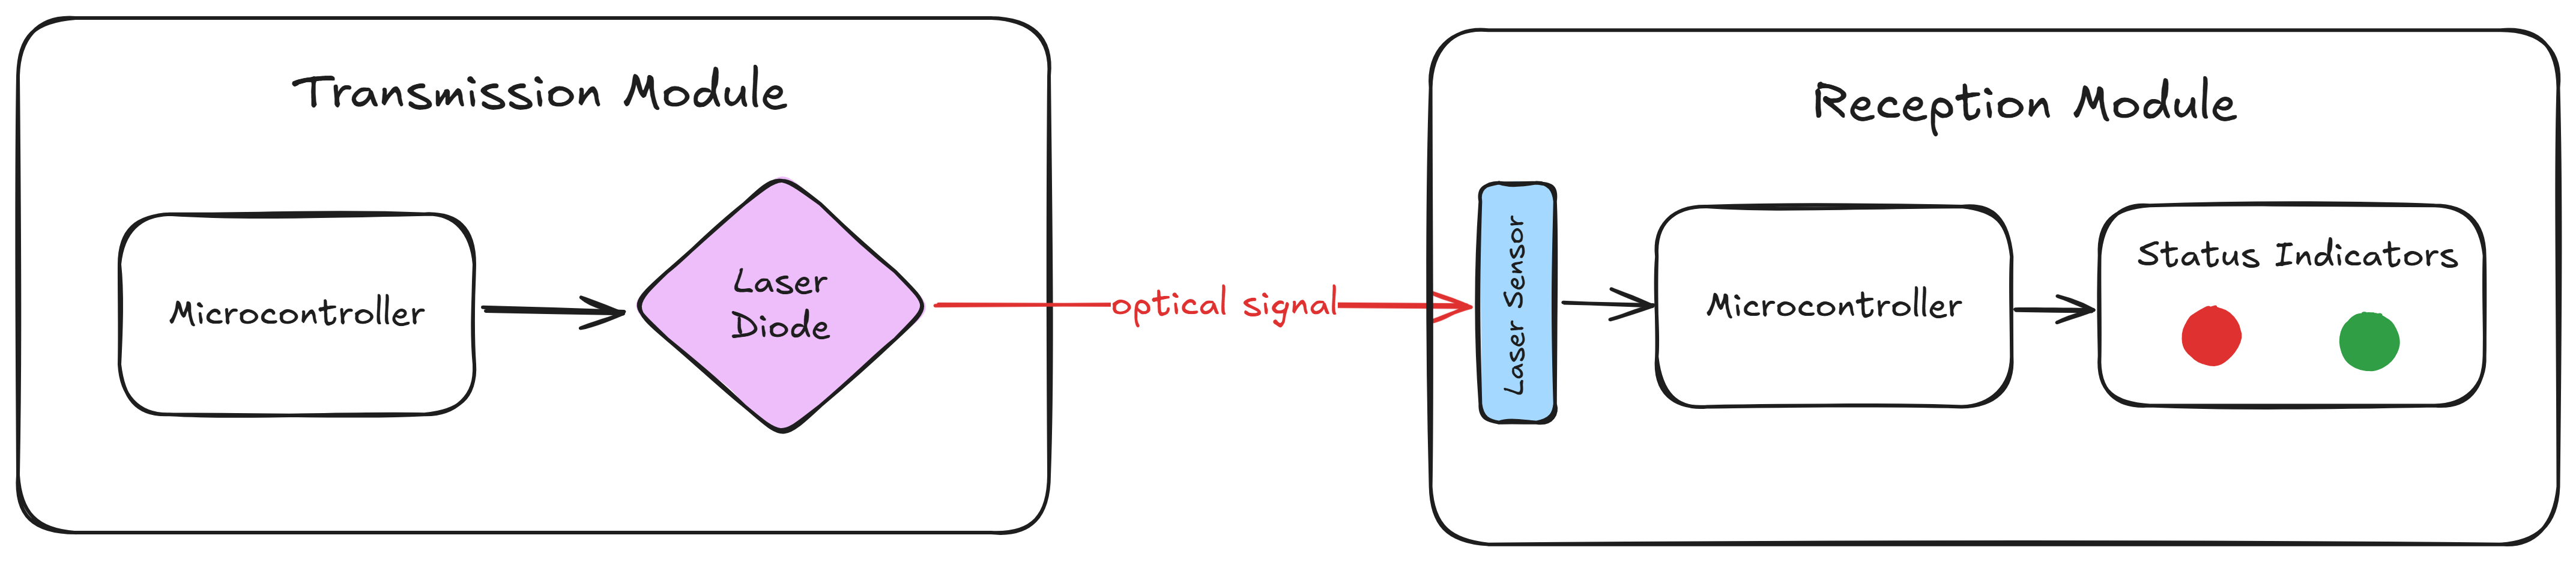
\includegraphics[width=0.8\linewidth]{flow_diagram.png}
    \caption{Signal Flow Diagram}
\end{figure}

\section{System Performance}
\subsection{Timing Optimization}
The system's timing parameters were optimized through iterative testing:

\begin{table}[h]
    \centering
    \begin{tabular}{lccc}
        \toprule
        Parameter & Original & Optimized & Improvement \\
        \midrule
        Pulse Width & 300ms & 100ms & 66.7\% reduction \\
        Bit Interval & 500ms & 200ms & 60\% reduction \\
        Total Sequence & 4.0s & 1.6s & 60\% reduction \\
        Debounce Time & 1000ms & 500ms & 50\% reduction \\
        \bottomrule
    \end{tabular}
    \caption{Timing Optimization Results}
\end{table}

\subsection{Reliability Considerations}
The system's reliability depends on several factors:
\begin{itemize}
    \item Line-of-sight maintenance between transmitter and receiver
    \item Physical stability of the mounting system
    \item Power supply stability
\end{itemize}

\section{Future Improvements}
Potential enhancements for the system include:
\begin{itemize}
    \item Implementation of error correction codes
    \item Support for multiple unique authentication sequences
    \item Integration of mechanical mounting solutions
    \item Development of a more compact form factor
\end{itemize}

\section{Conclusion}
This project successfully demonstrates a practical, contactless authentication system using modulated laser pulses. By employing readily available components and optimizing timing parameters, the system achieves reliable authentication with a significantly reduced processing time. This work validates the feasibility of low-cost optical authentication for access control and lays a foundation for future advancements in optical security technologies, such as increased security through more complex modulation schemes, integration with existing security infrastructure, and miniaturization for broader applicability.

\section{References}
\begin{enumerate}
    \item Arduino LLC. (2024). Arduino Official Documentation. 
    \item Fritzing. (n.d.). Fritzing: Software for electronics. Retrieved from https://fritzing.org/ 
\end{enumerate}

\appendix
\section{Appendix A: Circuit Diagram}

\subsection{Circuit Schematics}
\begin{figure}[h]
    \centering
    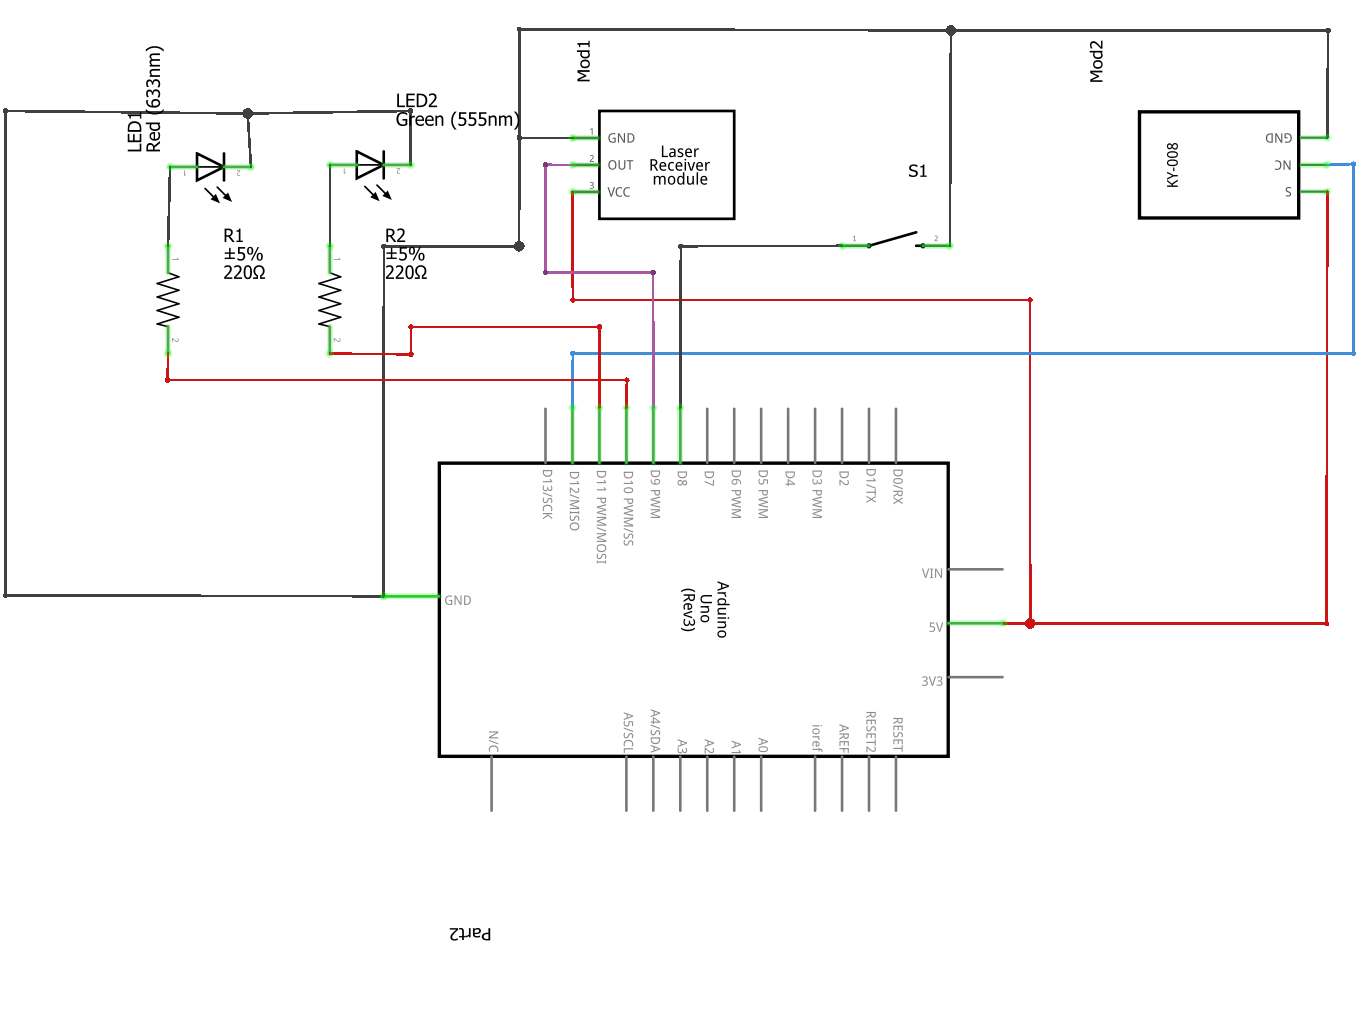
\includegraphics[width=0.59\linewidth]{schem.png}
    \caption{Circuit Schematics}
\end{figure}

\subsection{Circuit Connections}
\begin{figure}[h]
    \centering
    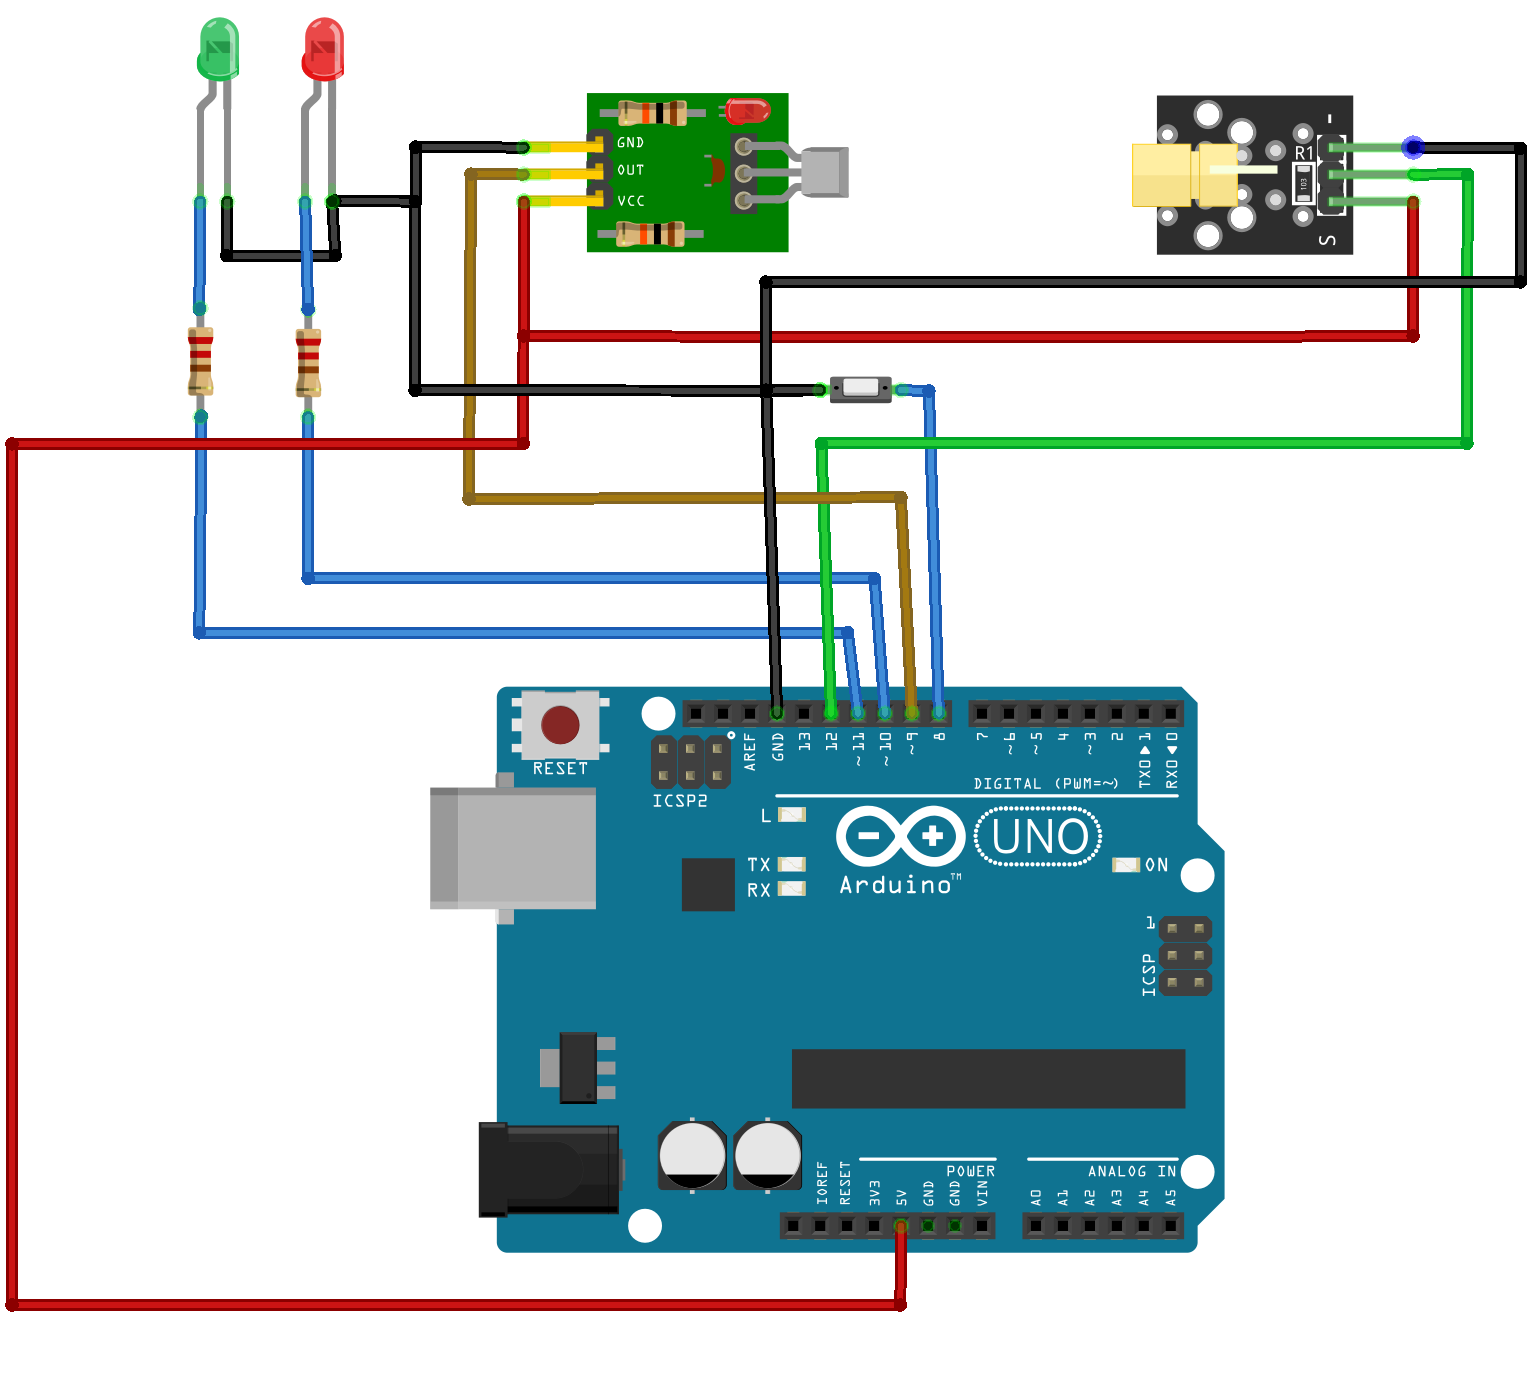
\includegraphics[width=0.5\linewidth]{bb.png}
    \caption{Circuit Connections}
\end{figure}

\section{Appendix B: Source Code}
The complete Arduino source code implementation\footnotemark[1]:
\begin{minted}{arduino}
const int laserPin = 12;     // laser diode
const int greenLedPin = 11;  // unlock indicator led
const int redLedPin = 10;    // lock indicator led
const int buttonPin = 8;     // push button pin
const int receiverPin = 9;   // laser receiver

const int inputSequence[] = { 1, 0, 1, 1, 0, 0, 1, 1 };
const int expectedSequence[] = { 1, 0, 1, 1, 0, 0, 1, 1 };
const int dataLength = sizeof(inputSequence) / sizeof(inputSequence[0]);
int receivedBuffer[24];  // circular buffer
int bufferIndex = 0;

// timing constants
const unsigned long pulseWidth = 100;
const unsigned long bitInterval = 200;
const unsigned long readInterval = 20;
const unsigned long debounceTime = 50;

// state variables
unsigned long previousMillis = 0;
unsigned long lastReadTime = 0;
unsigned long lastButtonDebounce = 0;
int dataIndex = 0;
bool transmitting = false;
bool isUnlocked = false;
int lastButtonState = HIGH;
int buttonState = HIGH;

void setup() {
  Serial.begin(9600);
  pinMode(laserPin, OUTPUT);
  pinMode(greenLedPin, OUTPUT);
  pinMode(redLedPin, OUTPUT);
  pinMode(buttonPin, INPUT_PULLUP);
  pinMode(receiverPin, INPUT);

  digitalWrite(laserPin, LOW);
  digitalWrite(greenLedPin, LOW);
  digitalWrite(redLedPin, HIGH);
}

void startNewTransmission() {
  transmitting = true;
  dataIndex = 0;
  Serial.println("\n=== Starting transmission ===");
  previousMillis = millis();
}

void handleButton() {
  int reading = digitalRead(buttonPin);

  if (reading != lastButtonState) {
    lastButtonDebounce = millis();
  }

  if ((millis() - lastButtonDebounce) > debounceTime) {
    if (reading != buttonState) {
      buttonState = reading;
      if (buttonState == LOW && !transmitting) {
        startNewTransmission();
      }
    }
  }
  lastButtonState = reading;
}

void checkReceivedSequence() {
  receivedBuffer[bufferIndex] = digitalRead(receiverPin);
  bufferIndex = (bufferIndex + 1) % 24;

  for (int start = 0; start <= 24 - dataLength; start++) {
    bool matched = true;
    for (int i = 0; i < dataLength; i++) {
      if (receivedBuffer[(start + i) % 24] != expectedSequence[i]) {
        matched = false;
        break;
      }
    }
    if (matched) {
      isUnlocked = !isUnlocked;
      digitalWrite(greenLedPin, isUnlocked);
      digitalWrite(redLedPin, !isUnlocked);
      Serial.println(isUnlocked ? "UNLOCKED" : "LOCKED");
      memset(receivedBuffer, 0, sizeof(receivedBuffer));
      bufferIndex = 0;
      break;
    }
  }
}

void loop() {
  unsigned long currentMillis = millis();

  handleButton();

  // transmit
  if (transmitting) {
    if (dataIndex < dataLength) {
      unsigned long timeSinceBitStart = currentMillis - previousMillis;

      digitalWrite(
        laserPin,
        timeSinceBitStart < pulseWidth &&
        inputSequence[dataIndex] == 1 ? HIGH : LOW
      );

      if (timeSinceBitStart >= bitInterval) {
        previousMillis = currentMillis;
        dataIndex++;
      }
    } else {
      transmitting = false;
      digitalWrite(laserPin, LOW);
    }
  }

  // receive
  if (currentMillis - lastReadTime >= readInterval) {
    lastReadTime = currentMillis;
    checkReceivedSequence();
  }
}
\end{minted}
\footnotetext[1]{This code represents the theoretical implementation of the system.}

\end{document}